\section{Introduction}
\label{sec:intro} 
Cellular networks are energy inefficient and consume several tens of TWhs of electrical energy
every year worldwide~\cite{Oh:Comm:2011}. This is a source of concern not only due to ecological concerns of global warming but also due to increasing operational expenditure resulting from rising fuel and electricity prices. 

In the present work, we focus on the second generation (2G) cellular network technology, Global System for Mobile communication (GSM). While most recent research focuses on later generations of cellular networks, we focused on GSM for the several reasons. First, it has a large consumer base. Second, upgrade to later generations of cellular networks is prohibitively expensive especially for operators in the developing world where profits are low due to cut-throat competition and return on investment is slow. Our proposed energy efficiency improvement framework is generic and should be applicable to other types of cellular networks as well, but we make no claim to its effectiveness in such scenarios. 

Within a GSM network, 50\% to 90\% of electricity consumption is at Base Transceiver Stations (BTSs)~\cite{Louhi:2007:BTSPower:INTELEC,Oh:Comm:2011}. Therefore, to reduce the electricity consumption in GSM networks, we focus on reducing the energy consumption at the BTSs.

In a GSM network, every BTS is equipped with several transceivers (TRXs), each of
which is allocated a single frequency band for transmission and
reception of radio signals. Each TRX further uses time
multiplexing to handle up to 8 full-rate voice calls over its
assigned frequency band in GSM systems. A typical configuration
is ``6+6+6'', depicting a BTS serving three \textit{sectors}
each with six TRXs. Thus, a BTS offers a \textit{fixed} capacity, as
determined by the total number of TRXs installed. Sites are
deployed such that this fixed BTS capacity can handle the peak
traffic load. However, traffic peaks only for a short duration
dropping off to a much lower trough each day, which means that
the GSM networks are over-provisioned during
low-traffic regimes.

Over-provisioned BTSs would be fine if they also
consumed little power at no traffic
load. However, according to~\cite{Peng:2011:BTSSaving:Mobicom}
the no-load power consumption can be as high as 95\% of that at
full load. With fixed BTS capacity that is over-provisioned for
low traffic loads, today's cellular networks are highly energy inefficient.

There are generally two approaches to improve cellular network
energy efficiency. First is a clean-slate redesign which includes
innovations in communication systems, circuits and components.
This approach is not attractive for existing GSM operators,
which are the most prevalent in the developing world and are
expected to stay as such for several years to come, primarily due to the required expensive upgrades. 
A second approach is to make optimizations to the existing system
and equipment to get an improvement in overall energy
efficiency. Our present work is aligned with this latter
philosophy.

One can improve the energy efficiency of a cellular network by
adapting its ``online'' capacity to changes in traffic load.
Recent work has proposed turning off base stations to reduce
energy consumption during times of low traffic
load~\cite{Louhi:2007:BTSPower:INTELEC,Oh:Comm:2011,Peng:2011:BTSSaving:Mobicom,He:CellularPower:JN:2012}.
However, our conversations with multiple network operators
indicate that they are reluctant to employ such techniques
citing three reasons:
\begin{itemize}
\item Power cycling of entire base stations is expected to
    reduce equipment life time.
\item Turning off some BTSs may require an increased uplink
    power which may not be handled by many low-cost/power-limited mobile
    stations (MSs). This raises a risk of customer churn and is
    not acceptable to the operators in cut-throat
    competition prevalent in today's market.
\item These techniques of turning off BTSs may
    underestimate the increase in power needed for indoor
    MSs.
\end{itemize}

Our conversations with
mobile network operators (MNOs) reveal that during low traffic periods, they often use a feature available in most vendor's equipment that deactivates TRX circuits at locations that
serve very few customers. Huawei calls this feature \textit{TRX shutdown} while Ericsson calls it \textit{BTS power saving}. We use the latter term generically in this paper. Since BTS power consumption has a traffic-independent
component~\cite{Peng:2011:BTSSaving:Mobicom} that depends,
among other factors, on the number of active TRXs, deactivating
TRXs reduces the BTS power consumption. For instance, turning
off one TRX cuts down BTS power consumption anywhere from $20W$
to $100W$, depending upon the frequency band (900 or 1800) and
deployed
equipment~\cite{Lorincz:BTS-Measure:Sensors:2012,flexibsc}.
Thus, scaling a ``6+6+6'' to a ``2+2+2'' configuration, by deactivating 12
TRXs will result in a saving of
240W to 1200W on a single site. The decision to use \textit{BTS
power saving} feature is generally local to the BTS without any
coordinated effort at the network level.

\begin{figure}
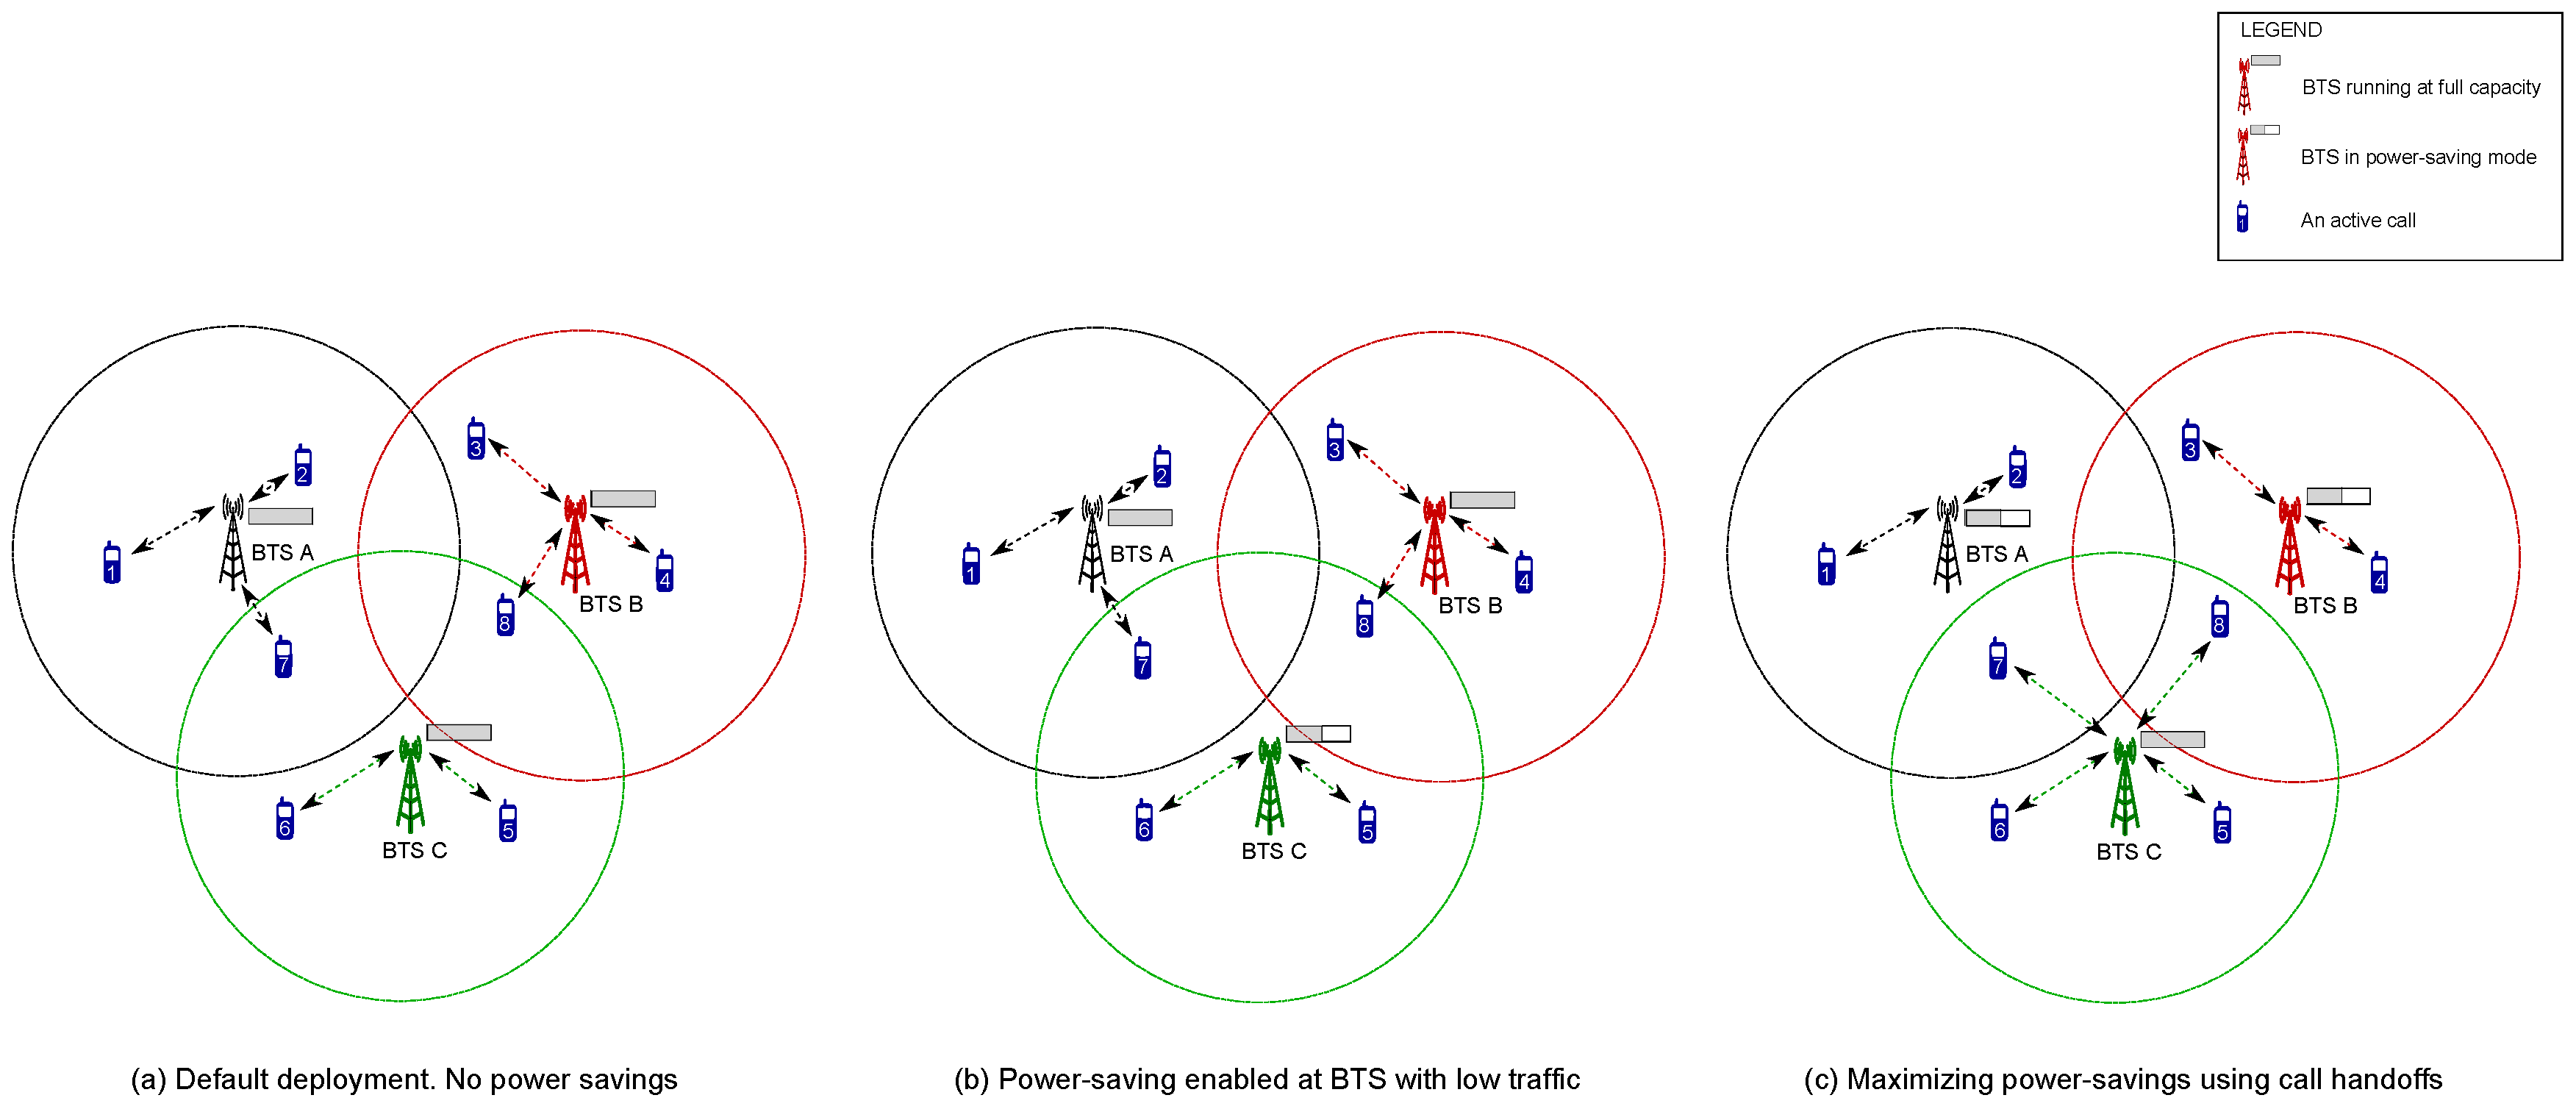
\includegraphics[width=1\textwidth]{figures/illustrationall.eps}
\caption{An example to illustrate the main idea behind Low-Carb. Three BTSs (A, B and C) are shown alongwith eight active calls. The serving BTS for each call is shown using arrows. A solid completely filled bar alongside a BTS symbol indicates that it is running in the default configuration whereby all TRXs are enabled. A BTS in power-saving mode is indicated with a half-filled bar next to it. Assume that power-saving mode may be enabled at a BTS if it has upto two active calls. (a) shows the default configuration where power-saving mode is not used. (b) shows the approach currently used by operators whereby power-saving mode is enabled on a BTS with low-traffic. (c) shows our proposed approach, whereby calls may be handed-off to nearby BTSs, thus maximizing the number of BTSs in power-saving mode.}
\label{fig:illustrationall}
\end{figure}


Let us illustrate the main idea behind the energy-saving approach proposed in this paper with the help of Figure~\ref{fig:illustrationall}. The figure shows three nearby BTSs collectively serving eight active calls. The association of call to the serving BTS is indicated by means of arrows, while the boundary of the potential service area of a BTS is indicated by means of a dashed circle around it. By default, each call is served by the BTS from which the mobile station receives the strongest signal. In this example, we assume that the call handling capacity of each BTS is six simultaneous calls. Furthermore, we assume that the power-saving threshold is two calls, i.e., if a BTS is serving upto two calls, it may be put into power-saving mode. In Figure~\ref{fig:illustrationall}, a BTS in its default configuration, i.e., all TRXs enabled is indicated with a solid bar next to the BTS symbol. Meanwhile, a BTS in power-saving mode is shown by a half-filled bar next to the BTS symbol.


In Figure~\ref{fig:illustrationall}, note that calls 1 through 6 each have only one candidate serving BTS, while call 7 may be served either by BTS A or C and call 8 may be served either by BTS B or C. Figure~\ref{fig:illustrationall} (a) shows the default deployment with default call routing whereas no power-saving is used. Since BTS C is serving only two calls, it may be placed in power-saving mode. Figure~\ref{fig:illustrationall} (b) shows this network state, which indicates the current practice in operational cellular networks, whereby BTS C is put into power-saving mode because its current call volume is below the power-saving threshold. However, this is not the optimal call routing strategy in terms of energy-savings. We may handoff calls 7 and 8 to BTS C, thereby reducing the call volume at both BTS A and B below the power-saving threshold. This results in the energy-optimal call routing strategy, proposed in this paper, shown in Figure~\ref{fig:illustrationall} (c). 


This paper presents Low-Carb which combines the \textit{BTS
power saving} with \textit{hand-off}, another commonly used
feature in cellular networks that facilitates user movement
from one location to another. Low-Carb proposes to hand-off
calls from one BTS to another, without making a negative impact
on the network quality of service, such that the \textit{BTS
power savings} can be applied to a maximal number of base
stations throughout the cellular network. As compared to the
use of uncoordinated \textit{BTS power savings}, Low-Carb
offers additional power savings as it may allow a larger number
of TRXs to be deactivated. 
In present day deployments, this is possible since most callers
receive sufficiently strong signal from several nearby
BTSs~\cite{Peng:2011:BTSSaving:Mobicom}. Fig.~\ref{fig:btscdf}
shows the coverage diversity evident in the urban data, from a large
cellular provider, that we used in our evaluations; one can see
that about half of the callers have 3 or more candidates for
serving BTS. Furthermore, neighboring sites can have different traffic loads at a given time. Fig.~\ref{fig:traffic}, for instance, shows normalized traffic at two neighboring sites in our dataset for a 24 hour period. Thus, some calls may be handed off from busy BTSs to nearby BTSs with lower traffic volume to increase the number of BTSs in power-saving mode.

\begin{figure}
\centering
\subfigure[]{
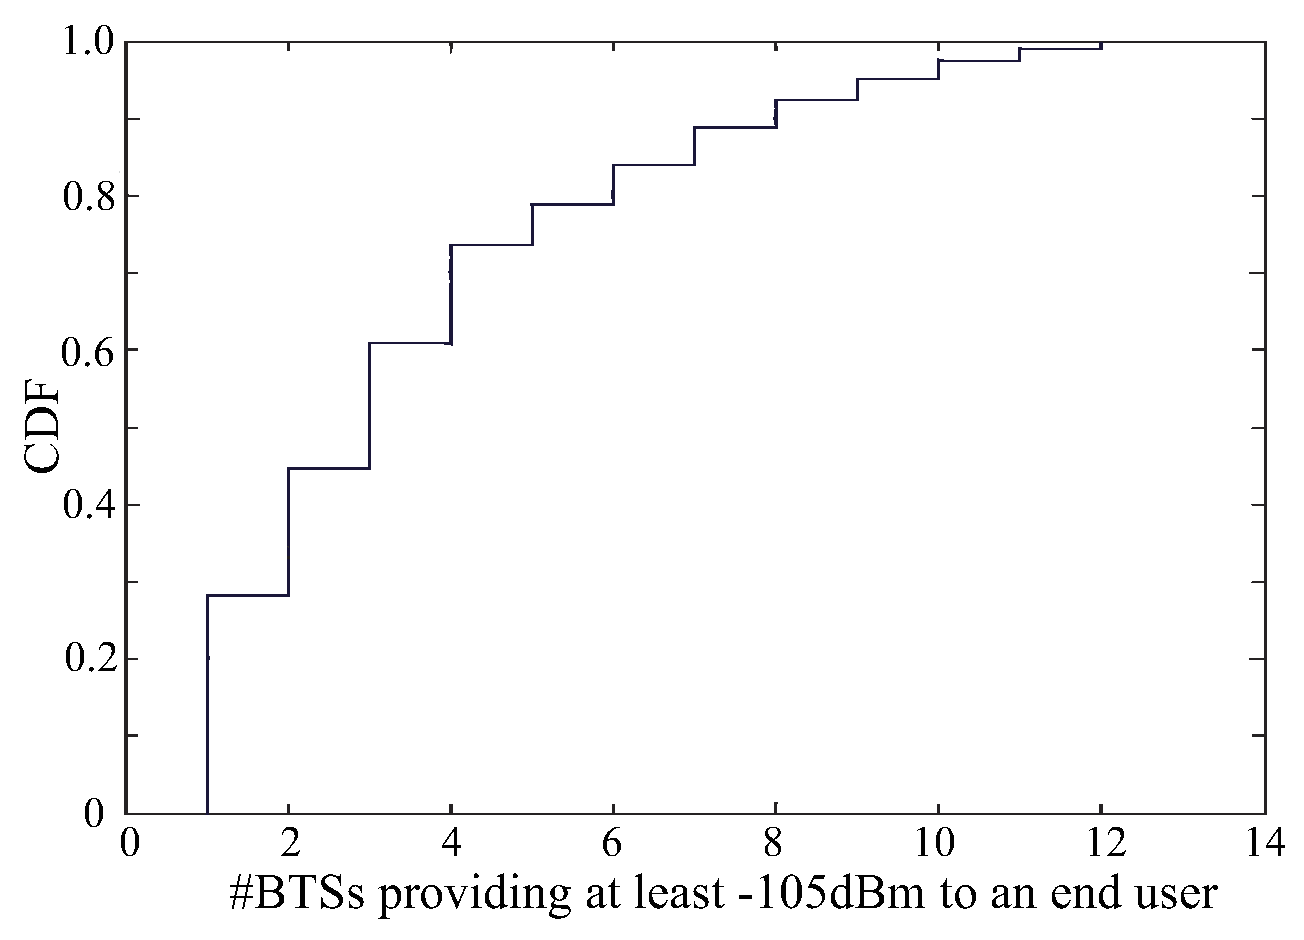
\includegraphics[width=0.48\textwidth]{figures/coveragecdf.eps}
\label{fig:btscdf}
}
\subfigure[]{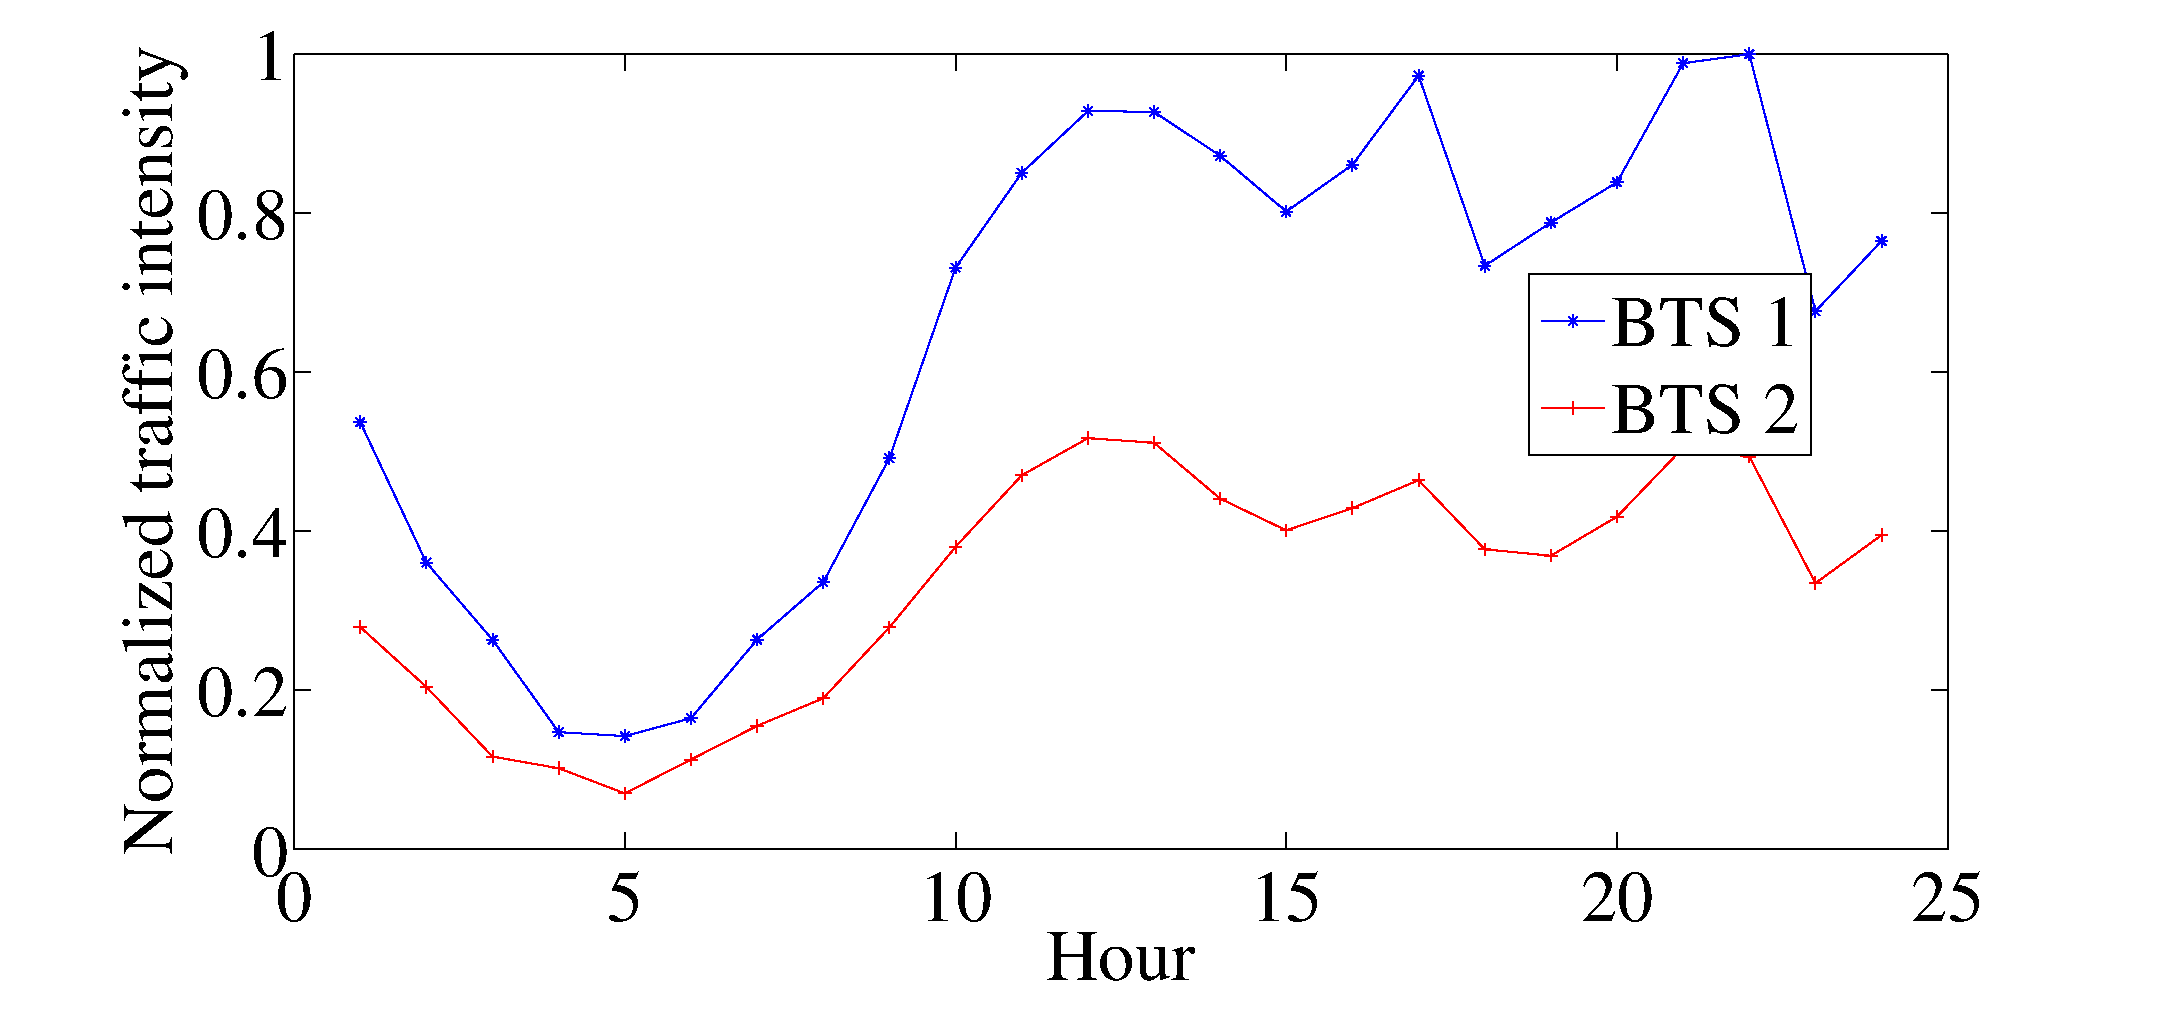
\includegraphics[width=0.48\textwidth]{figures/traffic.eps}
\label{fig:traffic}
}
\caption{Characteristics of our dataset: (a) Empirical CDF of the number of potential serving BTSs for a call in our dataset (large metropolitan area), (b) Normalized traffic intensity at two neighboring sites in our dataset} 
\label{fig:trafficmodelstats}
\end{figure}

We formulate an optimization problem to minimize the power
consumption in a GSM network by shuffling active calls between
nearby BTSs while keeping in check the MS uplink budget and without dropping any active calls. By constraining the uplink budget, we ensure that service quality is not adversely affected. 

In a shorter version of this paper~\cite{ilyas:lowcarb:globecom13}, we made the following contributions:
\begin{enumerate}
\item We formulated Low-Carb, a mathematical optimization problem to maximize energy savings in a cellular network such that call quality is not compromised. To maximize energy savings, Low-Carb relies on two features that are implemented in typical BTS hardware and are commonly used by cellular operators, albeit in an un-coordinated manner.
\item Since our formulation of Low-Carb is NP-Hard, we provided a heuristic algorithm for solving the Low-Carb problem.
\item We used real data sets from a large GSM network operator in Pakistan to evaluate Low-Carb's utility.
\end{enumerate}
In this paper, we extend our prior work to make the following additional contributions:

\begin{enumerate}
\item Let $\delta$ be the traffic capacity of the BTS in low-power mode. A BTS is placed in power-saving mode if its traffic reaches $\delta - \epsilon$ calls. If $\epsilon$ is chosen too high, then the energy savings will be low. On the other hand, if $\epsilon$ is chosen too low, then there may be several oscillations in and out of low-power mode due to short-term traffic variations. Rapid changes between a given pair of states are generally subject to damping because such changes are considered undesirable. We experiment with various values for $\epsilon$ and study the dependence of the amount of energy savings on the value of $\epsilon$.
\item In~\cite{ilyas:lowcarb:globecom13}, we had considered that a BTS could be put into one of two possible states, namely low-power and high-power mode. In this paper, we consider that a BTS may operate in one of six modes of operation in terms of its power consumption. We show that a higher granularity of number of BTS operational states results in greater energy savings.
\item We provide another heuristic algorithm for solving Low-Carb which is different from the one presented in the shorter version of this paper.
\end{enumerate}
The rest of the paper is structured as follows. In section~\ref{sec:related}, we summarize some of the related work. The formulation
of Low-Carb optimization problem is given in
section~\ref{sec:formulation}. Experimental setup and the
results are presented in sections~\ref{sec:expermintalsetup}
and~\ref{sec:results}, respectively. In
section~\ref{sec:conclusions}, we draw the conclusions
highlighting the power saving strategy for service providers.